\subsection{Paper Prototyping}\label{Sketches}
This section will include the processes of envisionment, evaluation and prototyping. The prototype is a paper prototype which means it consist of paper sketches depicting how the visual appearence of the program will be made. These sketches are fundamental ideas for the programs design but the design will most likely change during the development phase.

The navigation between the different windows of the program is done by using a bar in the bottom of the screen. This bar is always visible making it possible for the user to quickly select any of the main screens to navigate to. The bar is shown \cref{NavigationBarSketch}.

\subsubsection{Navigation bar}

\begin{figure}[H]
	\centering
    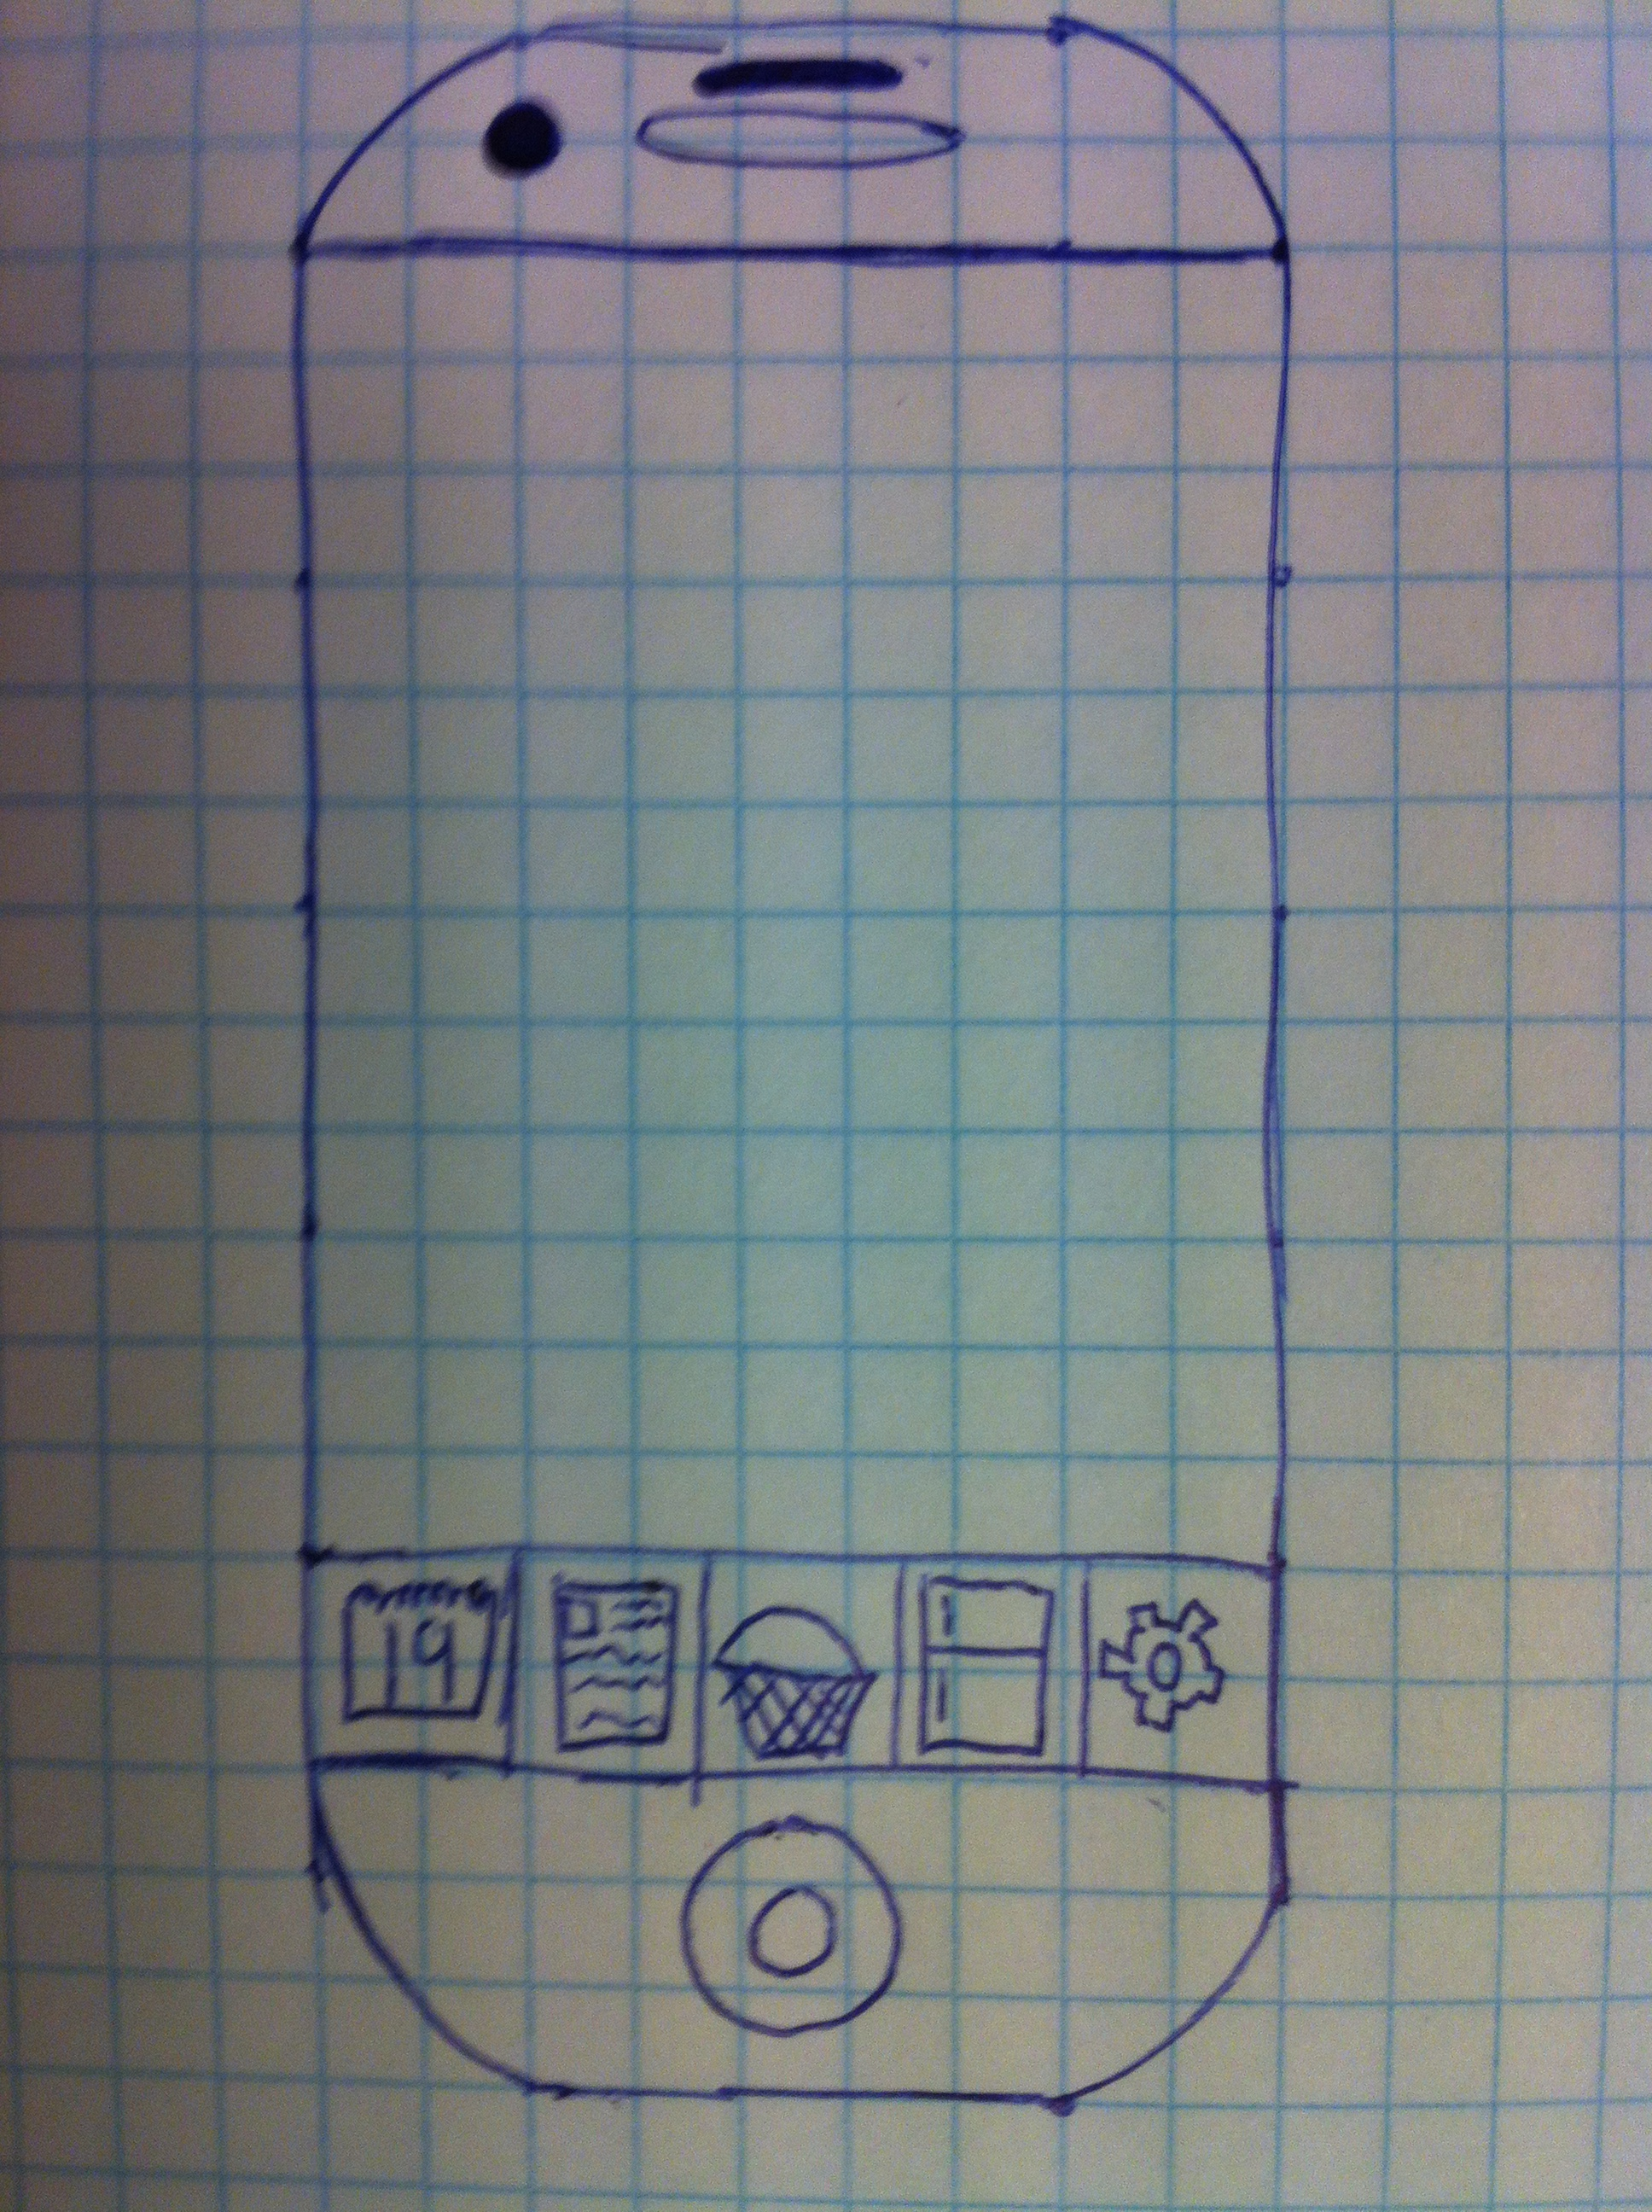
\includegraphics[width=0.5\textwidth]{Grafik/FoodPlanner/NavigationBarSketch}
	\caption{Navigation bar of the program, with the rest of the screen left blank}
	\label{NavigationBarSketch}
\end{figure}

The navigation bar is placed in the bottom of the screen. The bar has to be readable and its size therefore is quite dynamic as long as the readable requirement is satisfied. Depending on the screen size the navigation bar can fill up a large area of the screen. It has therefore been chosen that the bar will collapse downwards. When the bar is collapsed a line will be displayed at the bottom which the user can press on and the navigation bar will expand upwards.   

The navigation bar itself, consist of 5 buttons:

\begin{itemize}
    \item Meal plan
    \item Recipe
    \item Shopping list
    \item Inventory
    \item Settings
\end{itemize}

Each of the buttons take the user to the screen which it represent, and all of these screens will be described later in this section. The icons which are used in the representation are just for the design progress, and not necessarily the final ones.

\section{Meal plan}
\subsubsection{Recipe} \label{RecipesSketches}
In this section the recipe screen is going to be described. Both the functionality of the screen and the design principles used in the design process are going to be described. The sketch used to illustrate the use consist of two different screens, one screen only showing a full screen of the recipe, and one screen showing how to browse through the recipe. The browsing screen is divided into two sketches, showing the functionality of this screen.

The image sketches referred to can be seen in \cref{FinalRecipeBrowsingSketch2} and in \cref{FinalRecipeBrowsingSketch1}. The sketch in \cref{FinalRecipeBrowsingSketch1} is the first screen to see, when browsing recipes. The right screen in \cref{FinalRecipeBrowsingSketch2} shows the expanded version of the recipe browsing screen, and the left shows the full screen of the recipe.

\begin{figure}[H]
    \centering
    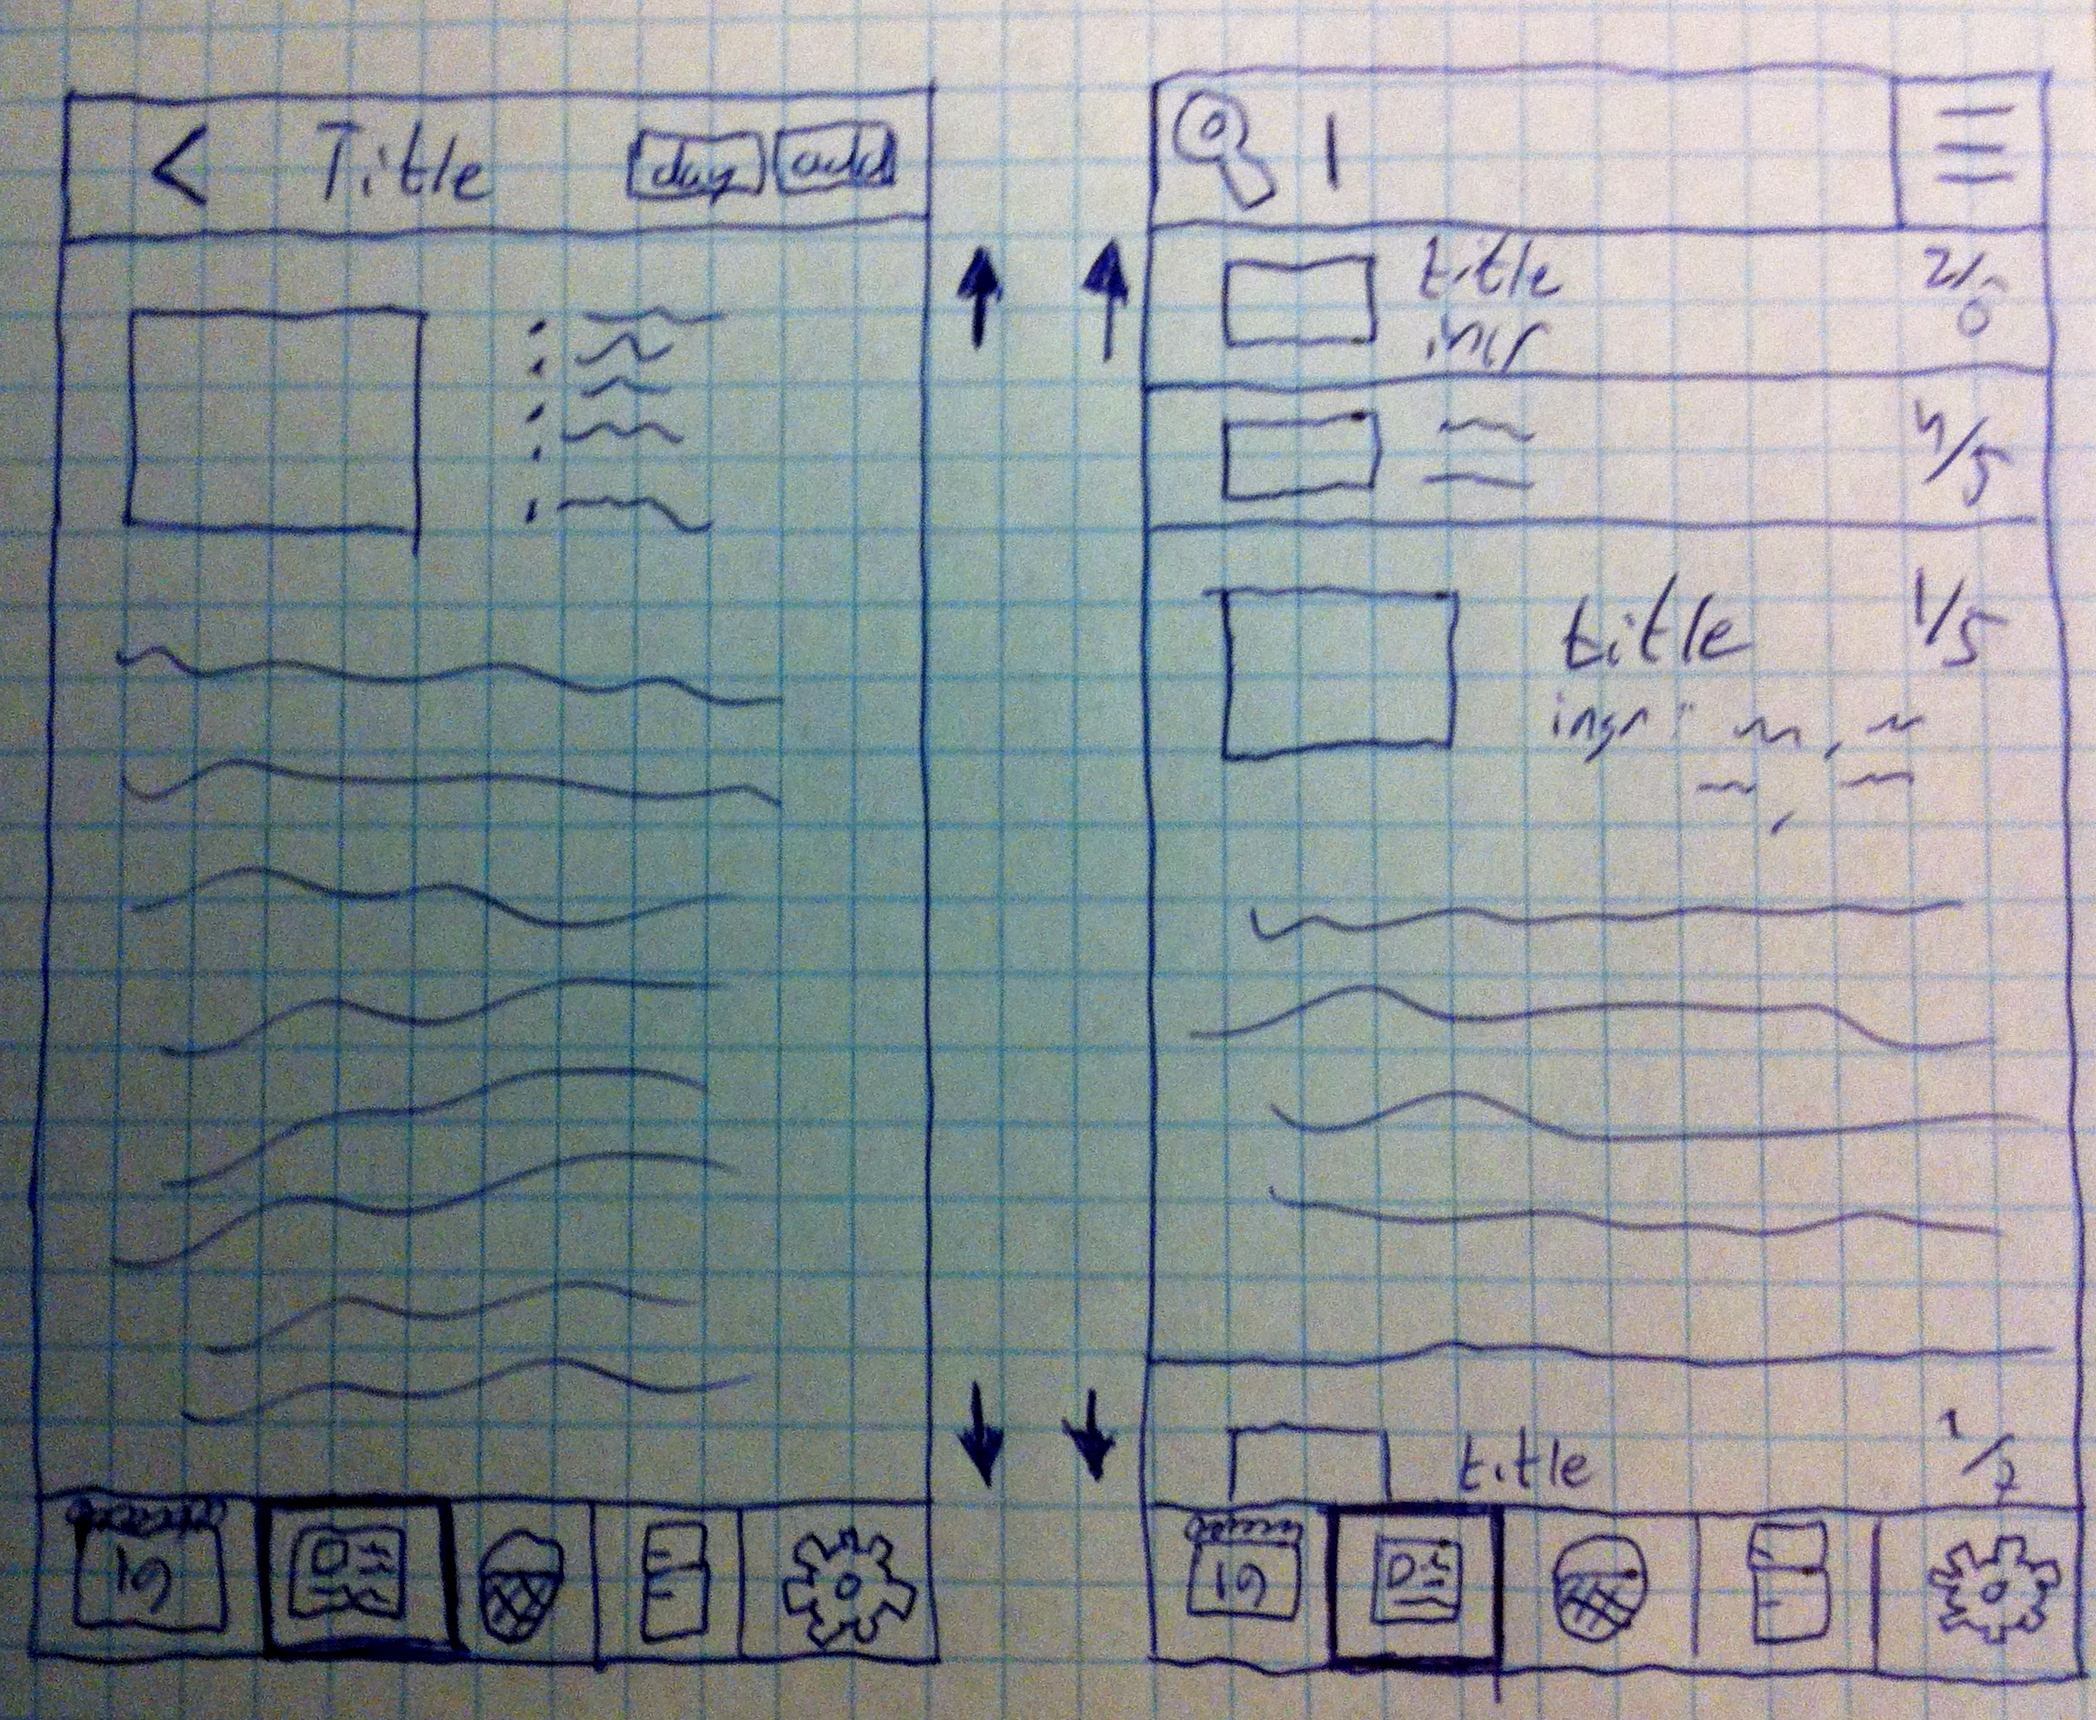
\includegraphics[width=0.5\textwidth]{Grafik/FoodPlanner/FinalRecipeBrowsingSketch2}
    \caption{One of the final sketches of the recipe browsing screen.}
    \label{FinalRecipeBrowsingSketch2}
\end{figure}

\textbf{Two screen idea:} Looking at the recipe browsing screen (right sketch on \cref{FinalRecipeBrowsingSketch2}) there are three elements to explain: 

\begin{itemize}
    \item Search bar
    \item Sort button
    \item List of recipes
\end{itemize}

The search bar is located on the top of the screen, as it is where the user is most likely to look for it at first, since this is where most search bars in mobile applications, but also websites, is located. When text is entered into the search bar, the recipes containing the text will be shown in the list of recipes. 

The sort button offers the user the functionality of sorting the list of recipes by different requirements. It might be by time to cook, by number of ingredients the user already has in the inventory, or by something else. The sort button is located at the right side of the search bar, as this was a convenient place to position it. It only consists of an icon showing that you will be able to sort the recipes by clicking the button.

The list of recipes show the recipes that the user can choose from. These are sorted by the sort button, or the search bar previously described. If there are more recipes available than the screen can display, the user will be able to swipe in an upwards motion for more recipes to appear at the bottom and the recipes at the top will disappear. In the right side of each recipe it is shown how many of the ingredients needed to make the recipe the user already have; an example is if the user has 4 out of the 10 ingredients needed the right side will show "4/10".

Looking at the specific recipe screen (left sketch on \cref{FinalRecipeBrowsingSketch2}) there are two elements to explain:

\begin{itemize}
\item Top navigation bar
\item Recipe viewing area
\end{itemize} 

The expanded recipe screen can be seen in \cref{FinalRecipeBrowsingSketch2} on the right. It is similar to the recipe browsing screen, but this screen shows more information about a specific recipe.

When the user has chosen a recipe, the user will be able to click it. By doing so, the recipe will expand, and more information about the recipe will be shown. This will only be the most relevant information, such as ingredients, cooking time, and a picture.

\begin{figure}[H]
    \centering
    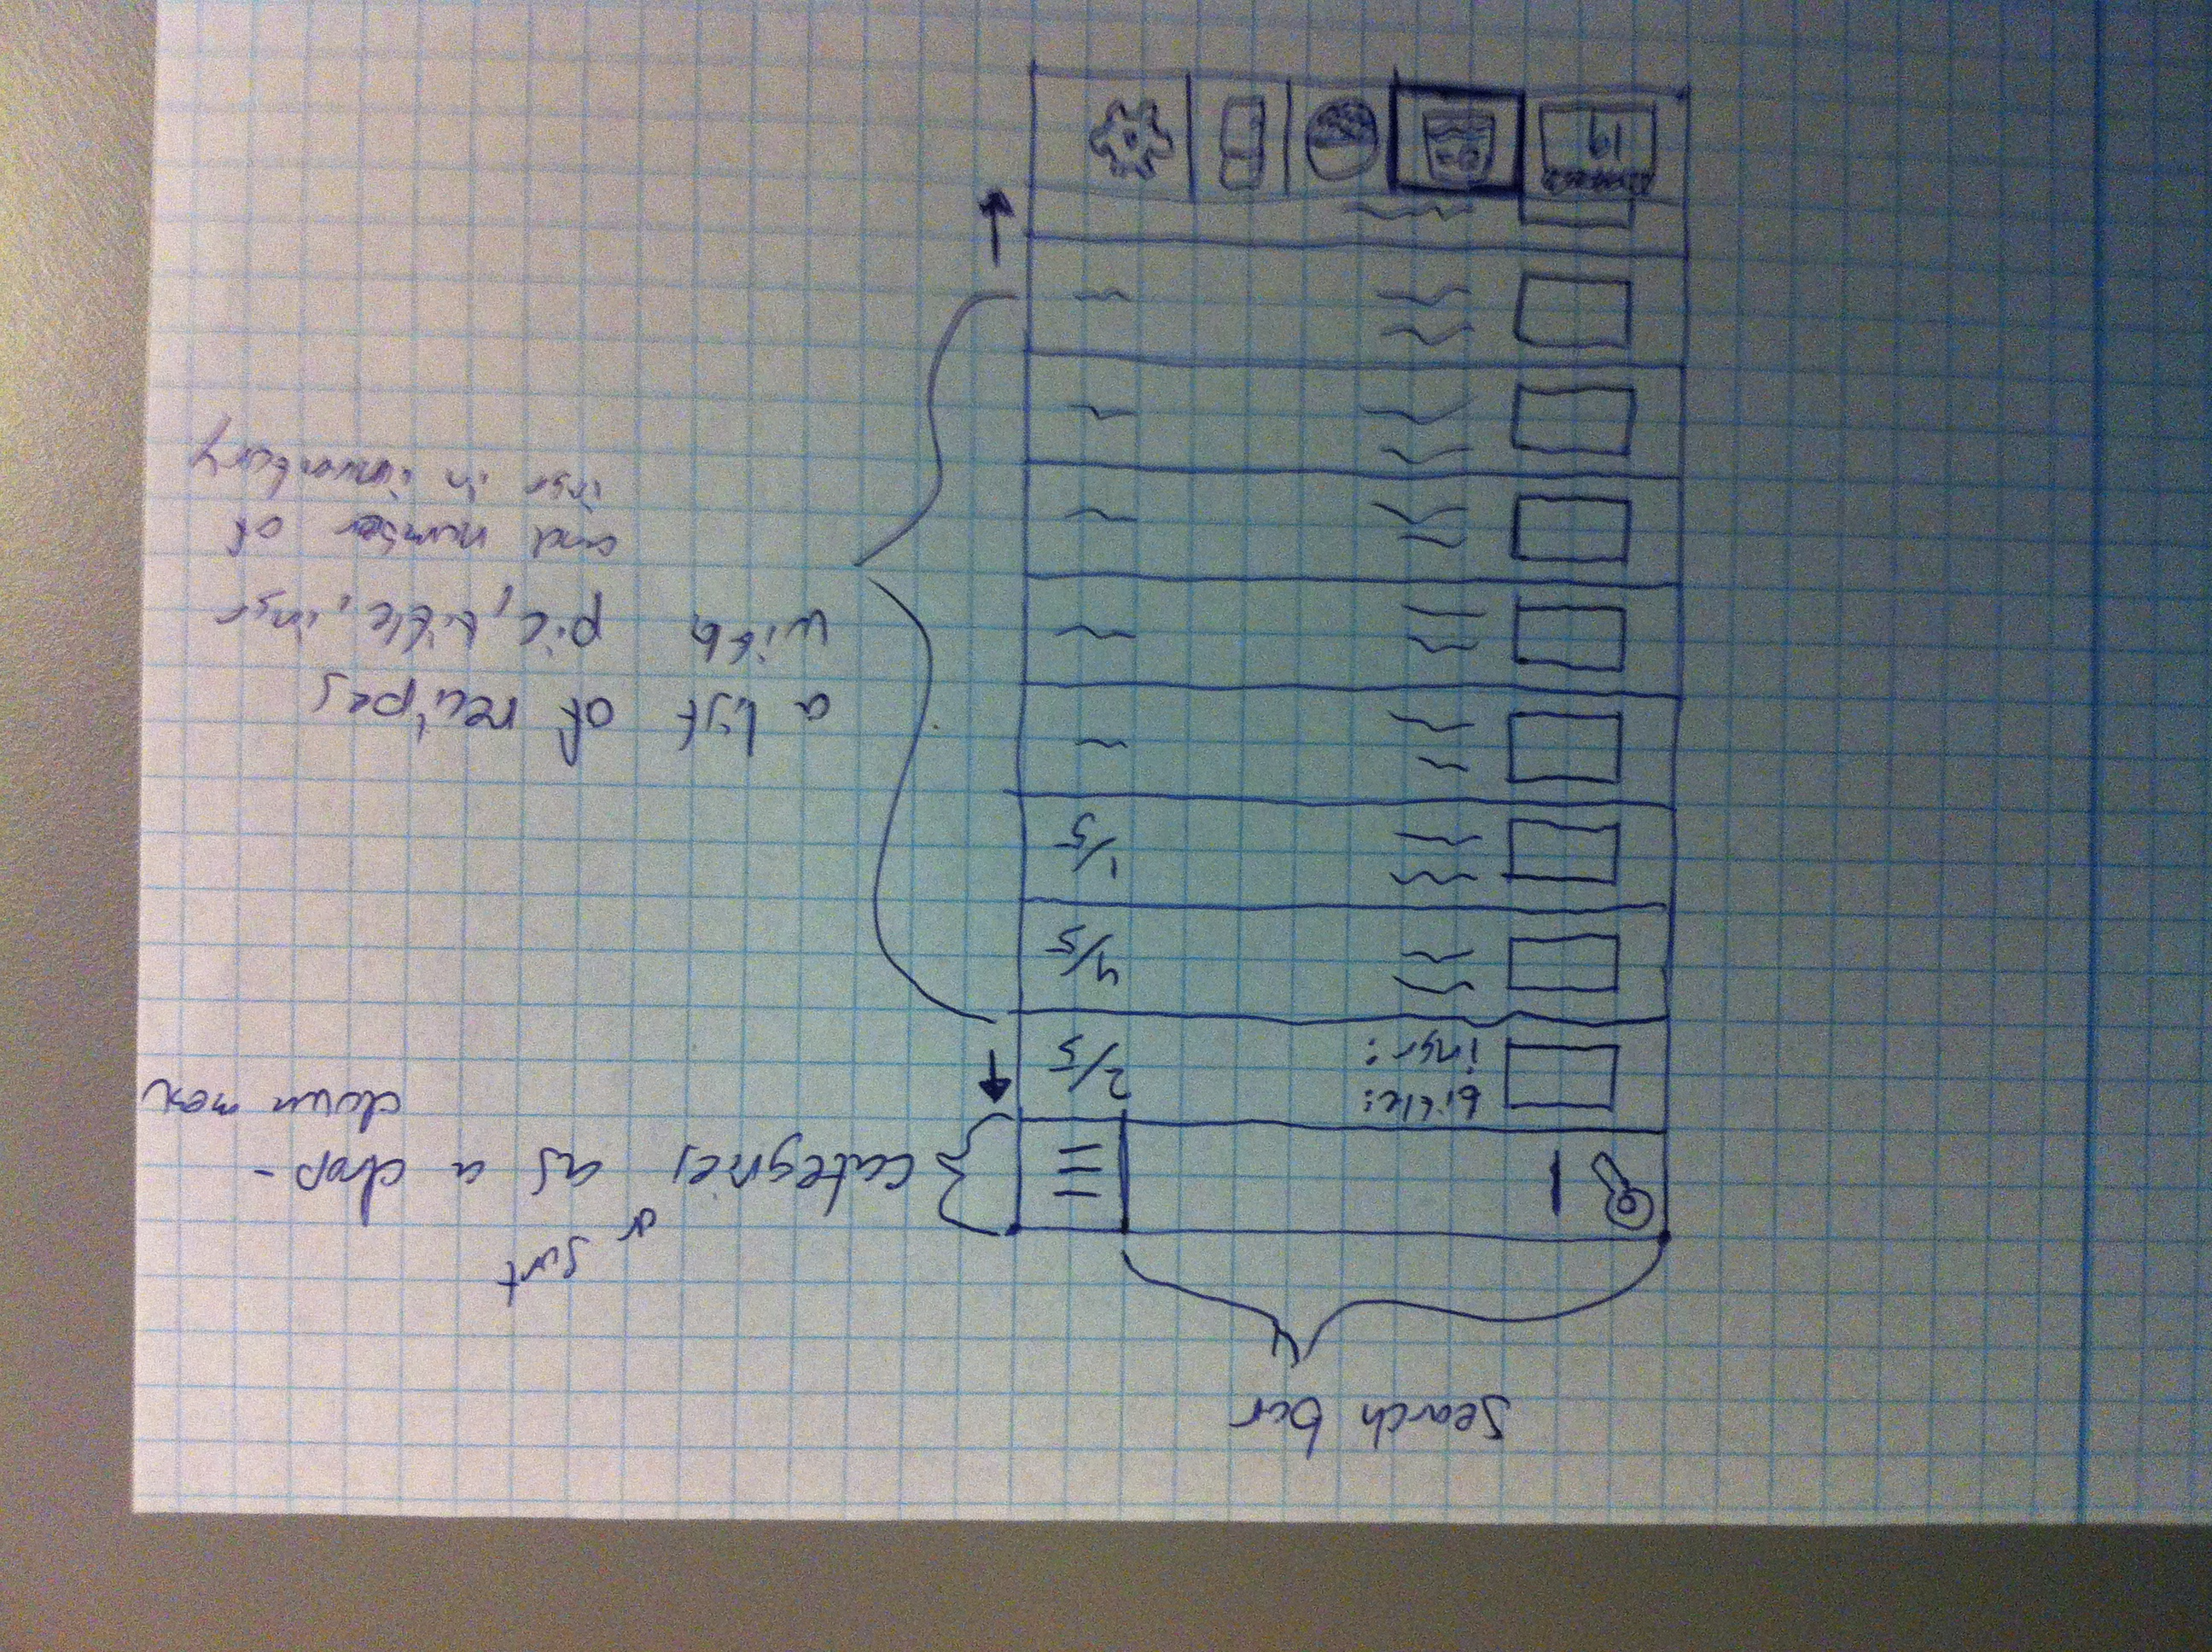
\includegraphics[width=0.5\textwidth]{Grafik/FoodPlanner/FinalRecipeBrowsingSketch1}
    \caption{One of the final sketches of the recipe browsing screen.}
    \label{FinalRecipeBrowsingSketch1}
\end{figure}

\textbf{Full screen recipe screen:} The full screen recipe screen is the left sketch on \cref{FinalRecipeBrowsingSketch2}. This screen gives the full overview of the recipe.

On the left side, a picture of the recipe will be shown if available, and the ingredients will be listed on the right side of the picture. Beneath the ingredient list, instructions on how to prepare the meal are shown. If the recipe is longer than the amount of text the screen can hold, the user will be able to scroll through the rest of the recipe by swiping.

In the top of the screen there is a navigation bar. This navigation bar gives the user the ability to do three things:

\begin{itemize}
    \item Go back
    \item Change the amount of people attending the meal
    \item Add the recipe to the meal plan
\end{itemize}

The arrow in the left of the navigation screen indicates a go back function, giving the user the ability to go back to the recipe browsing screen, if the user did not want to do anything further with the shown recipe.

The second element enables the user to change the amount of people attending the meal. This would change the amount of ingredients needed in the recipe, and would also update the shopping list, so the user would buy the right amount of the ingredients needed.

The last button gives the user functionality to add the recipe, being viewed, to the meal plan. This would update the shopping list, and add the meal to a specific day chosen by the user.
\subsection{Inventory} \label{InventoryScreen}

In this section the sketch of the inventory screen is going to be described. The functionality is going to be described as well as the design principles used in the design process. The sketch consists of 3 sketches of the screen, describing 3 different states of the inventory screen as can be seen in figure \ref{FinalInventorySketch}. The first screen from the left, shows the screen when no action has been taken. The second screen from the left shows an expanded ingredient. The third screen from the left shows the screen when the user is searching for an ingredient.

\begin{figure}[H]
    \centering
    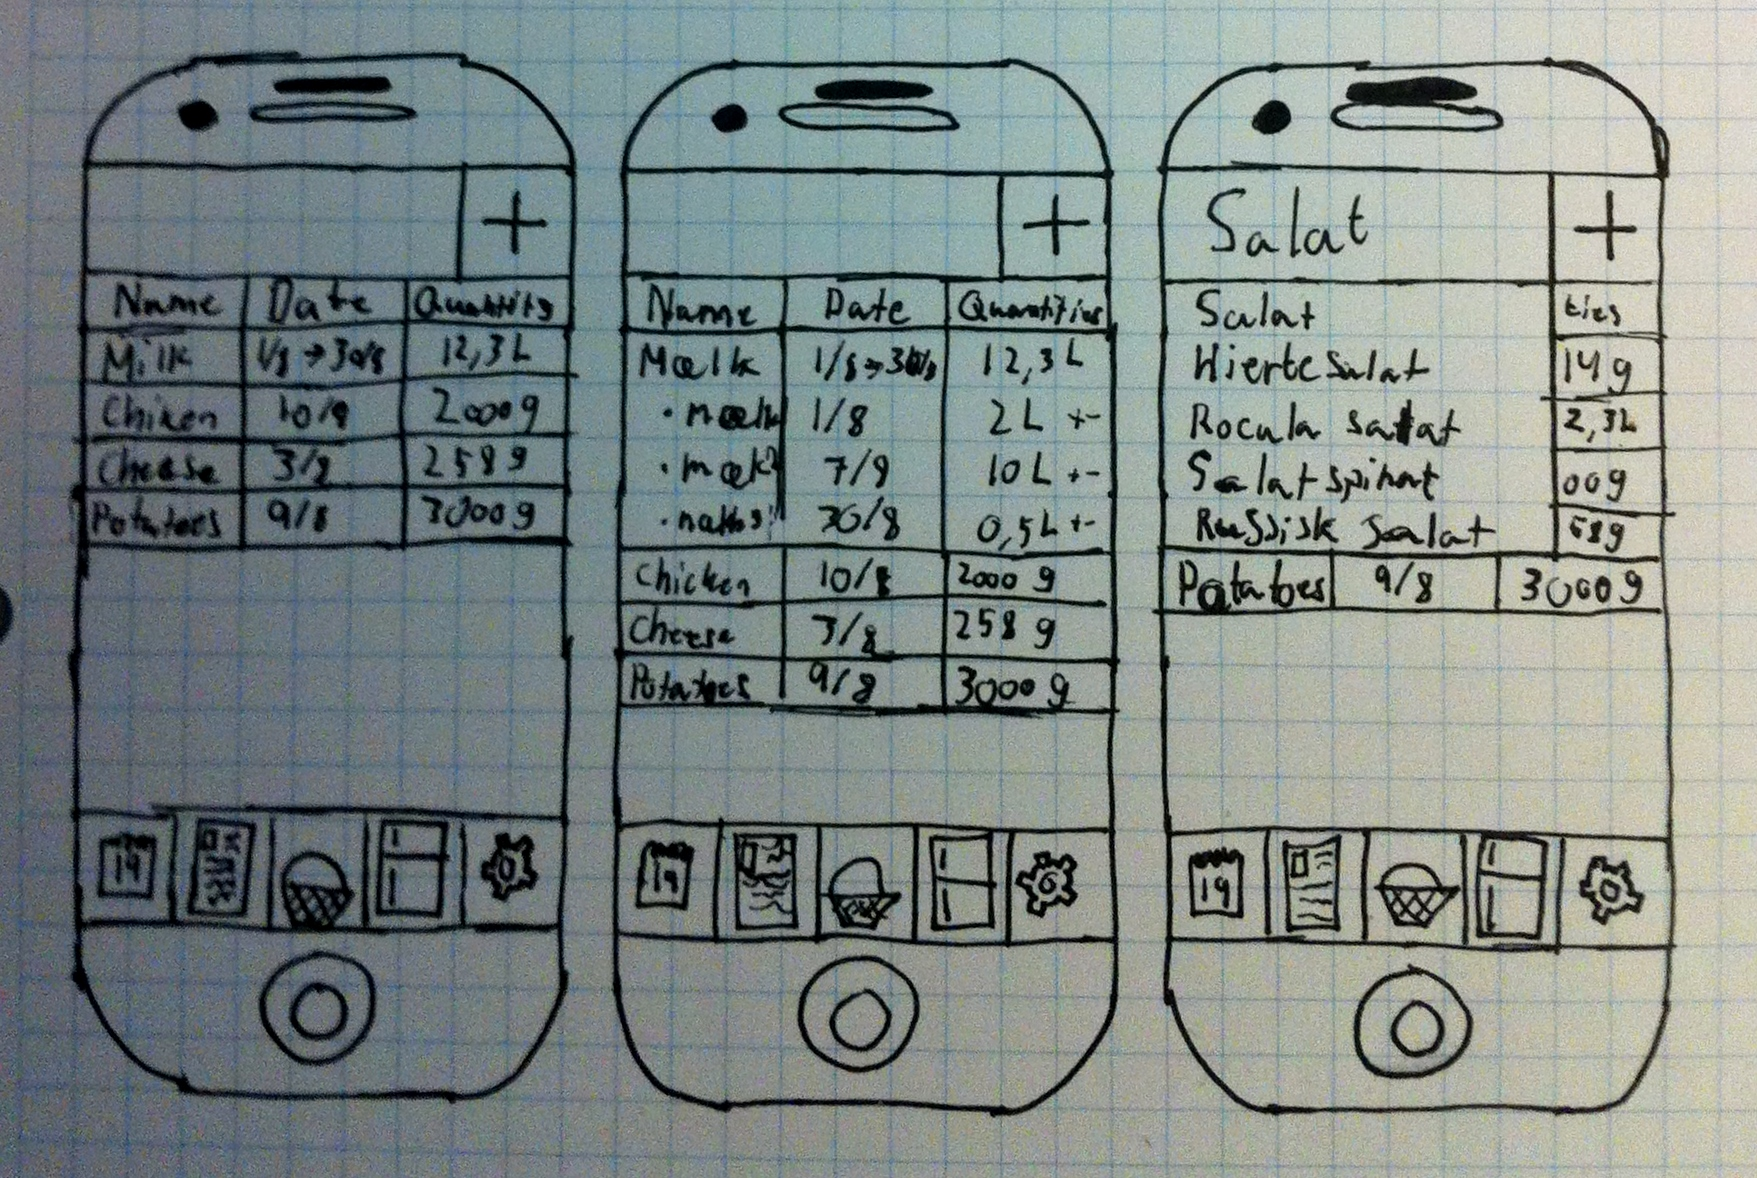
\includegraphics[width=0.5\textwidth]{Grafik/FoodPlanner/FinalInventorySketch}
    \caption{The final sketch of the inventory screens}
    \label{FinalInventorySketch}
\end{figure}

\subsection{Inventory overview screen}

The inventory overview screen is divided into two different elements, not taking the general design elements into consideration. These elements are:

\begin{itemize}
    \item Search bar
    \item Table
\end{itemize}

The search bar is placed in the top of the screen, as this is where a user most likely will look for it first, because on most mobile applications and also on websites, the search bar is located at the
top of the screen. The add icon is used to make the user able to add items to the inventory, that are not included in the ingredients of the meal plan.

The second element is the table, which is located under the search bar. The table is divided into three columns; name of the item, expiration date of the item, and the quantity of the item.

The first column with the name of the item only holds the information about the items name. The second column shows the expiration date of the item, if the user only have one instance of the item, meaning that there will only be one expiration date, only one expiration date is shown in the expiration date column, but if the user has more instances of an item and therefore different expirations dates, the first and the last expiration dates of the item will be shown, and an arrow in between the dates will indicate that the expiration dates go from the first to the last. The quantity column holds the information about the quantity of the item.

\subsection{Expanded ingredient list}

When the user click on an ingredient, the ingredient will expand and show all the instances of the information as shown on the second screen from the left in figure \ref{FinalInventorySketch}. The information is still stored in the three columns described in the inventory overview screen. An instance of the ingredient will therefore show the name of the instance, the expiration date and the quantity of the instance. 

\subsection{Searching for an ingredient}

The third screen from the left in figure \ref{FinalInventorySketch} shows the search function of the screen. When text is entered into the search box, the items in the search function will expand and lay over the ingredients in the inventory.

The search new overlay will show a fixed number of ingredients which has the searched text in their names, and the user can by clicking one of the ingredients, the expanded search bar will contract, and the item chosen will be shown in the search bar. By clicking the add icon the user will now be able to add the item to their inventory, and if the item already is in the inventory, the item will be an instance that the user can expand to see. The expiration date will then be changed in the table, as well with the quantity.
\subsubsection{Shopping list}

In this section the sketch of the shopping list is going to be described. The sketch is made up of two different screens, as seen in figure \ref{FinalShoppingListSketch}. One of the screens indicate the overview of the items on the shopping list, and the other screen shows the screen when something has been typed into the search bar.

\begin{figure}[H]
    \centering
    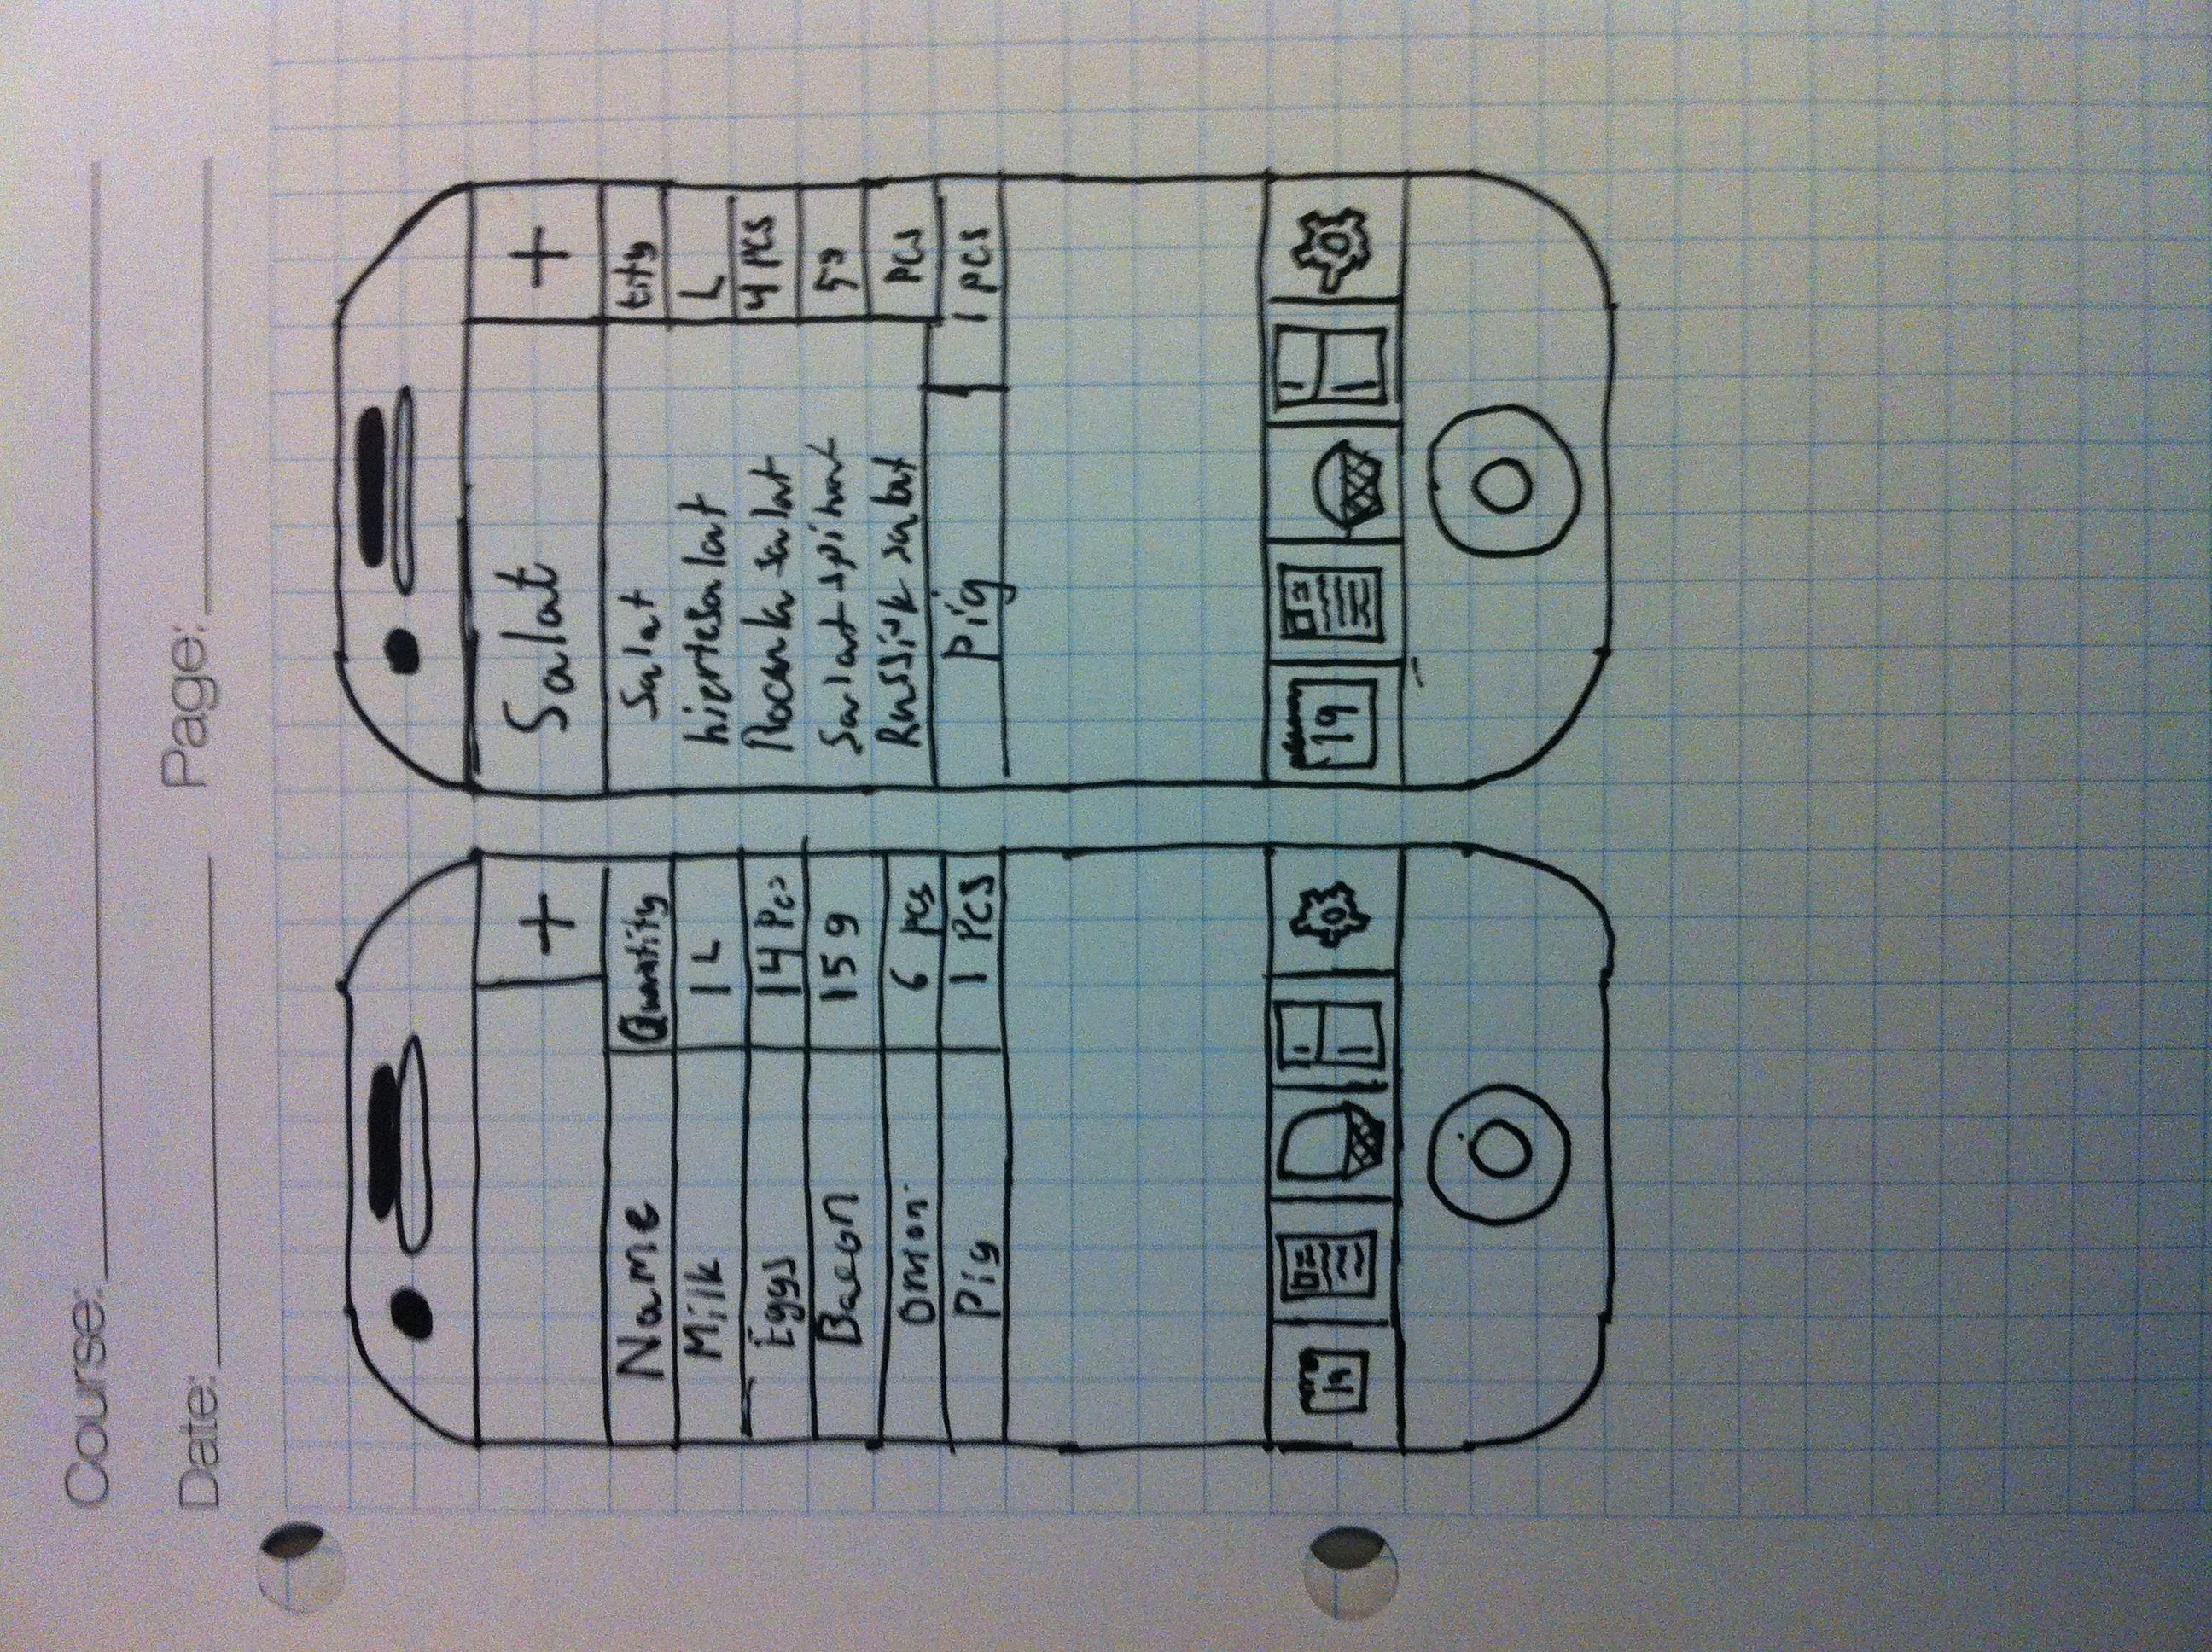
\includegraphics[width=0.5\textwidth]{Grafik/FoodPlanner/FinalShoppingListSketch}
    \caption{The final sketch of the shopping list screens}
    \label{FinalShoppingListSketch}
\end{figure}

\paragraph{Shopping List Overview screen}

The left screen in figure \ref{FinalShoppingListSketch} is the overview of the shopping list. This screen consists of two elements, not counting the general program elements, the elements is:

\begin{itemize}
	\item Search bar
	\item Table
\end{itemize}

The search bar is placed in the top of the screen, as this is where a user most likely will look for it first, because on most mobile applications and also on websites, the search bar is located at the top of the screen. The add icon is used to make the user able to add items to the inventory, that are not included in the ingredients of the meal plan.

The second element of this screen is the table, which is divided into two columns, one showing the item name, and one showing the quantity of the item. The column showing the name is broader, as the name of some items will be larger than the space needed to write the quantity.

The rows of this screens shows the ingredients on the shopping list, in the sketch, five ingredients is on the shopping list, though there could be as many as needed. If the number of different ingredients fills more than the screen can hold, the user would be able to scroll through the list by swiping upwards. Even though the user would wipe through the ingredients, the first row containing the text "Name" and "Quantity", would still be the first row.

\paragraph{Shopping List Searching Screen}

The second sketch (right sketch on \ref{FinalShoppingListSketch})  is showing the screen, when a search is performed. The screen will not change, but the search bar will expand and lay over the rest of the screen.

When a search is performed it will show a number of ingredients, in the sketch it is five, and all ingredients containing the word that have been searched for will be shown. Then the user will need to choose the ingredient they want to add to the shopping list, and click on the plus icon to add it to the list.

When a new item is added, it the user will need to go down to the quantity field, and put in the quantity of the item that will be needed.
\subsubsection{Settings}

The settings sketch can be seen in \cref{SettingsScreen} and are divided into 2 sketches. The left sketch show the list of settings, and the right sketch show the list of settings, with a specific sketch expanded.

\begin{figure}[H]
	\centering
    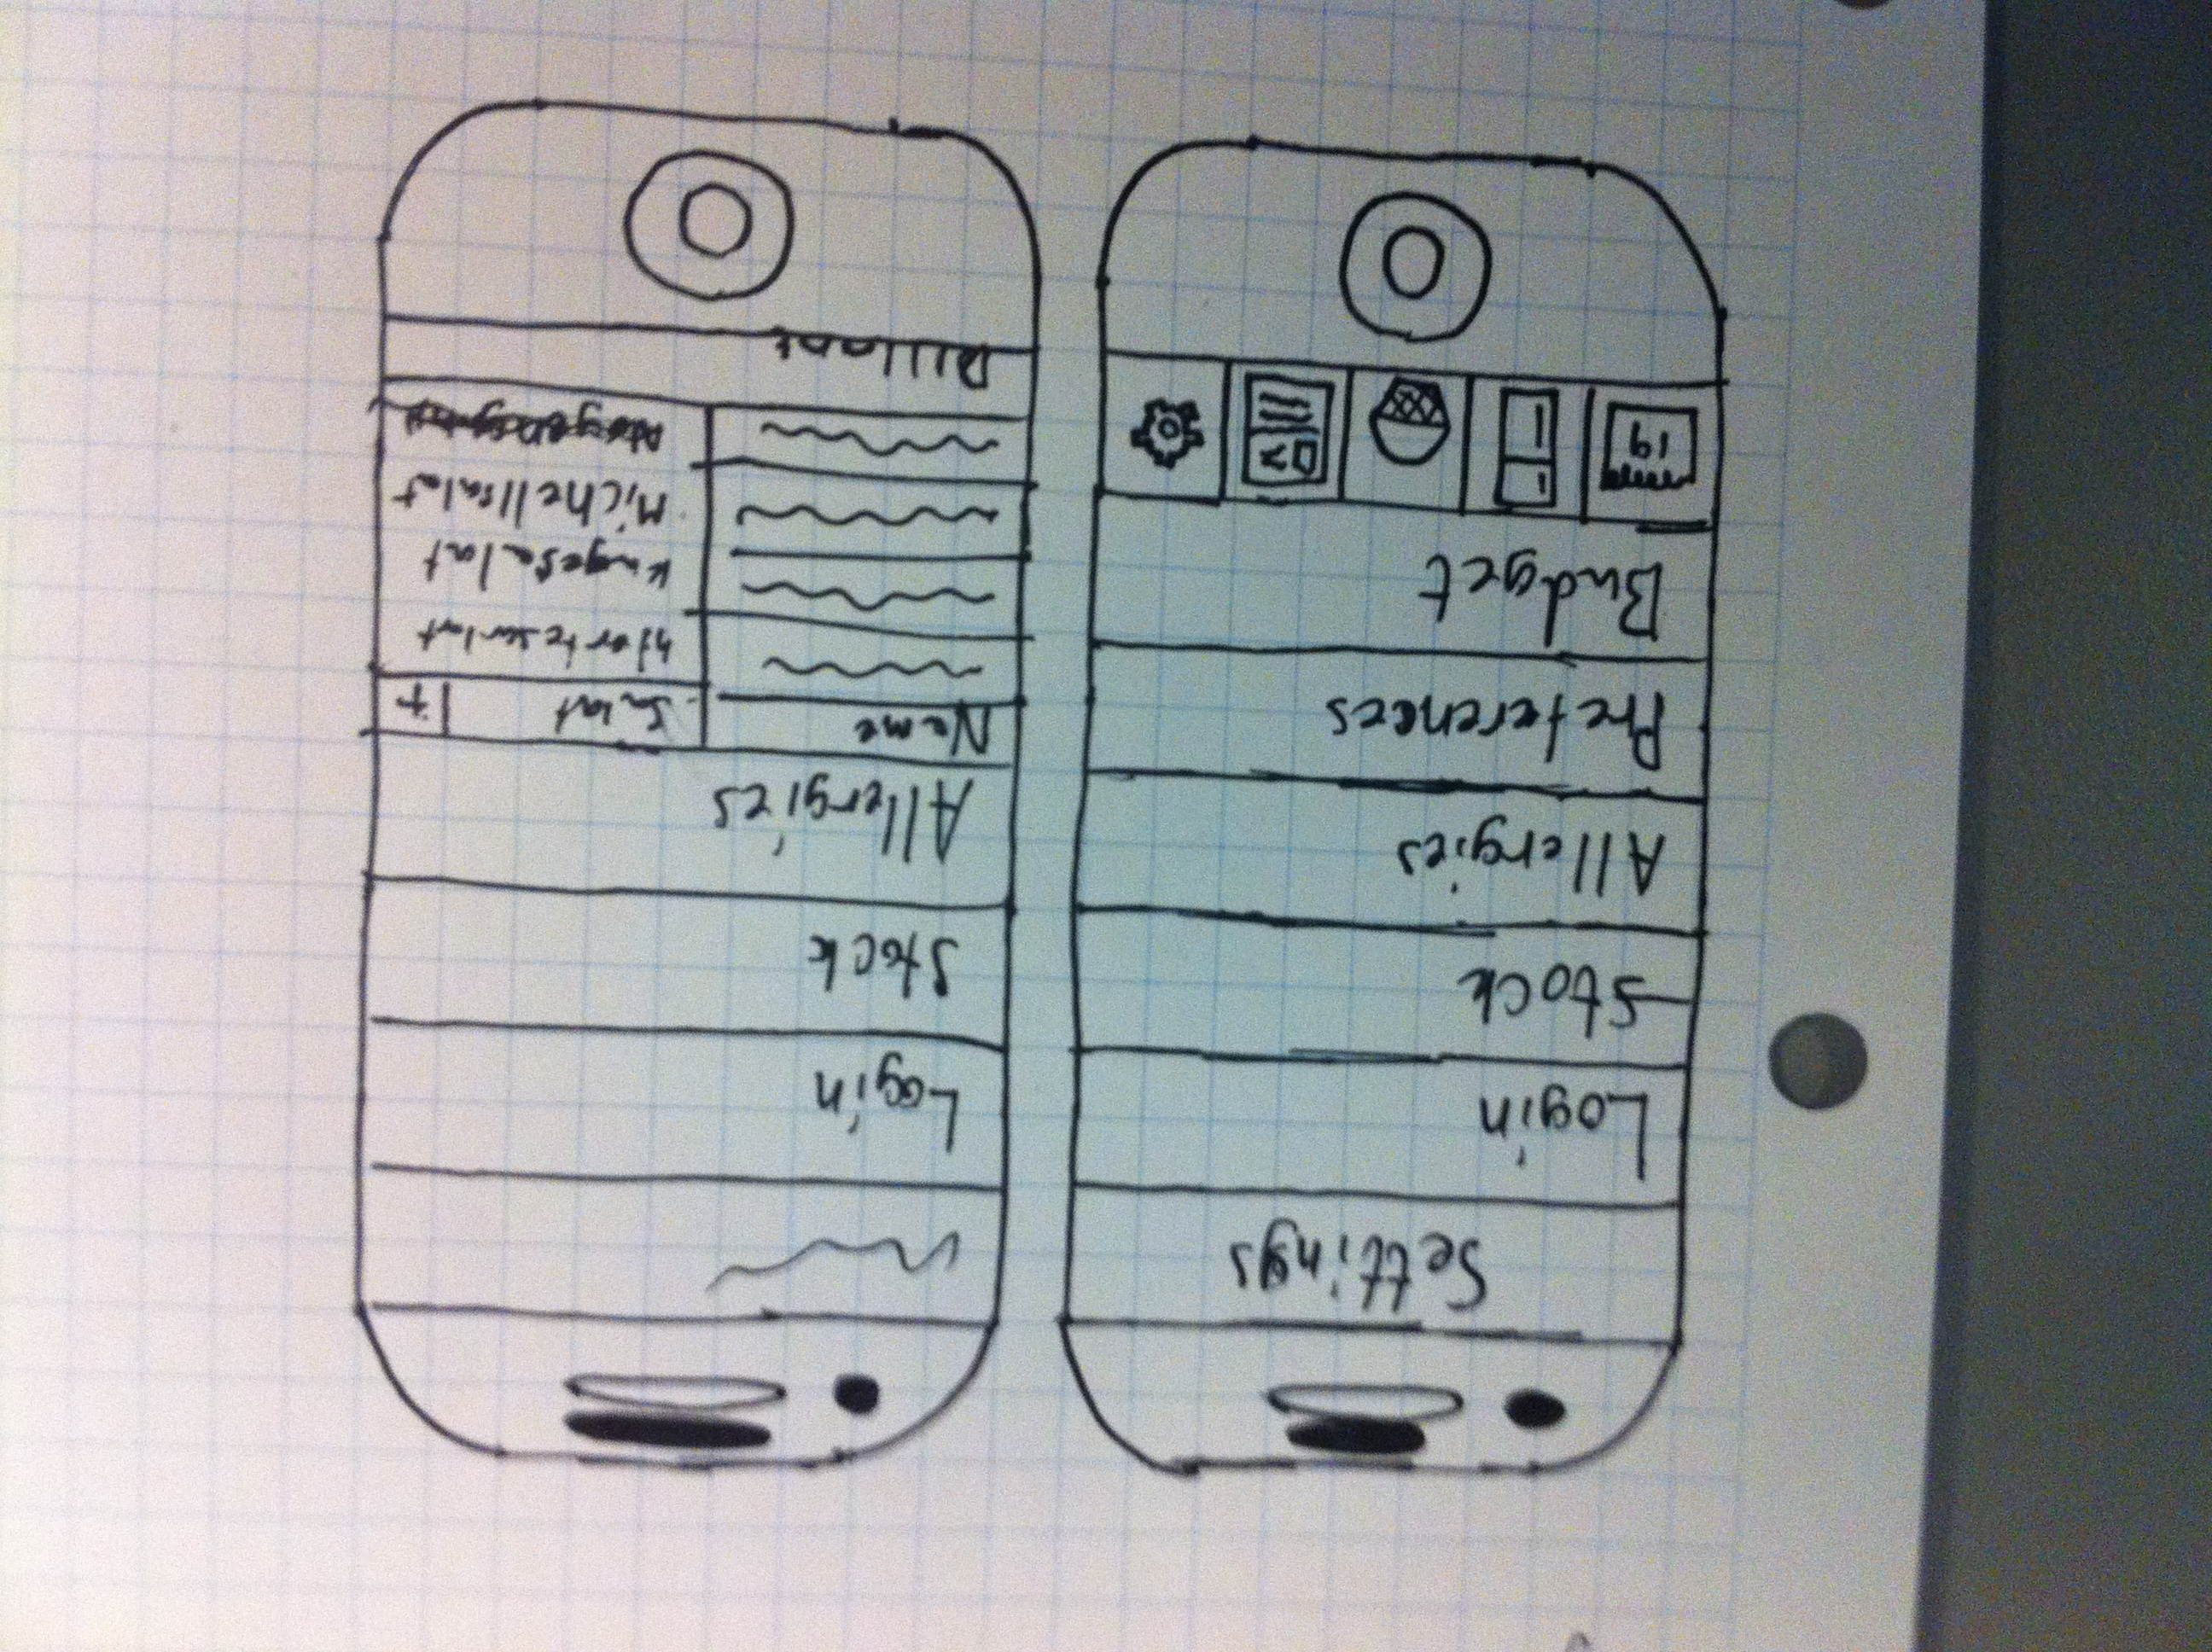
\includegraphics[width=0.5\textwidth]{Grafik/FoodPlanner/FinalSettingsSketch}
	\caption{This screen displays all of the settings in the program.}
	\label{SettingsScreen}
\end{figure}

\paragraph{Settings List} \label{SettingsList}

The setting list is the left sketch in \cref{SettingsScreen} and show a list of settings. The settings can be scrolled through, by swiping up and down, if more settings are needed than the screen can hold. The items shown in the sketch are just ideas for settings, and are just used to visualize the design idea. These are not all settings that will be incorporated in the program.

\paragraph{Expanded Settings List}

The right sketch in \cref{SettingsScreen} show the list of settings, as described in \cref{SettingsList}. Furthermore, this sketch has an expanded setting. This is because if a user click a setting,  it will expand, and show more information about this setting. In the sketch, allergies is expanded.

Expanding was chosen, because it would be consistent with the rest of the program, instead of other ideas that where discussed, for example a pop up. 
\subsubsection{Navigation diagram}
\Cref{NavigationDiagram} shows all of the screens that we have found so far through the evaluation of the concrete scenarios. These screens will be sketched in the next section of the report and the content and design considerations of each screen will be specified.  

\begin{figure}[H]
	\centering
	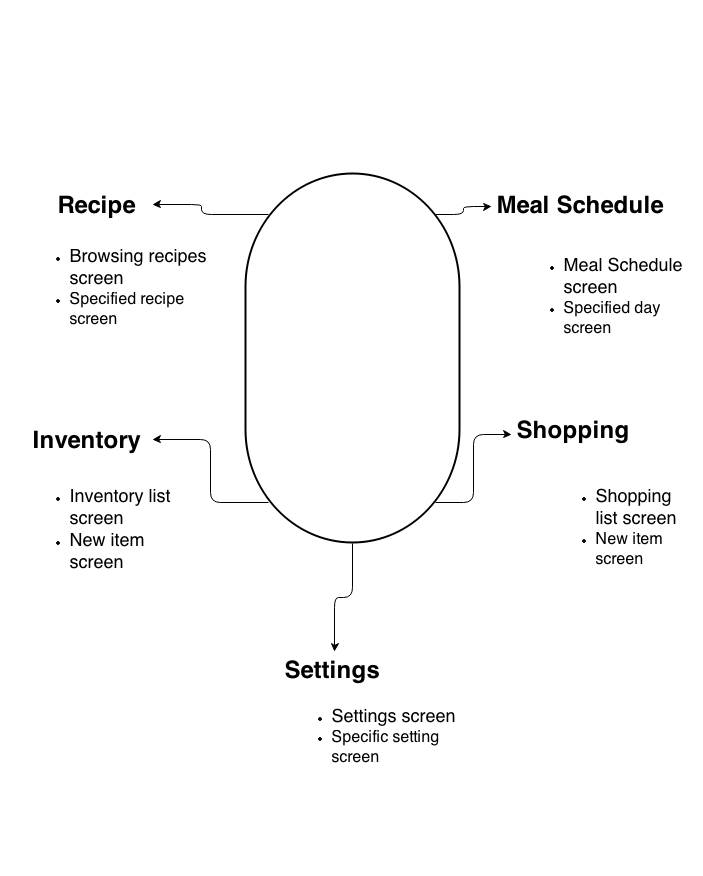
\includegraphics[width=0.8\textwidth, trim=0 3cm 0 5cm]{Grafik/FoodPlanner/NavigationsDiagram}
	\caption{This figure shows a navigation diagram for the different screens that have been uncovered in the evaluation process.}
	\label{NavigationDiagram}
\end{figure}
